%!TEX root = ../../prace.tex

\section{Počáteční inicializace projektu}

Pokud je cílem spustit projekt hry ze zdrojových kódů, je potřeba si stáhnout \UE{} ve verzi \TT{4.15.3}. Na hlavní stránce \UE{} je potřeba stáhnout \textit{Epic Games Launcher} (ke stažení zde~\citep{ue_download}). Po vytvoření uživatelského účtu a~následnému přihlášení do aplikace bude vidět obrazovka podobná obrázku \ref{fig:ueLauncher}:


\begin{figure}[!ht]\centering
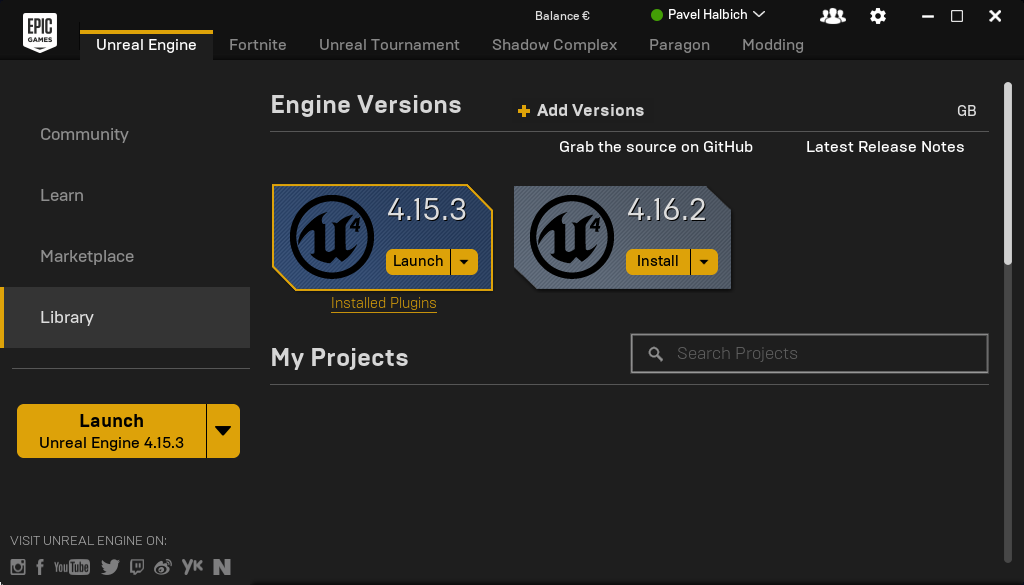
\includegraphics[ width=140mm]{../img/program/ueLauncher}

\caption{Epic Games Launcher}
\label{fig:ueLauncher}

\end{figure}

\FloatBarrier

Pokud není vidět \UE{} dané verze v~seznamu verzí, je potřeba jej přidat kliknutím na tlačítko \textit{Add Versions} a~případném následném výběru správné verze. Na obrázku \ref{fig:ueLauncher} je vidět \UE{} verze \TT{4.16.2}, který je připravený ke stažení. Posledním krokem je samotná instalace stisknutím tlačítka \textit{Install}. Použití novější verze \UEu{} je možné, ale běžnému uživateli to nedoporučujeme. Mezi verzemi se mohou projevit nekompatibility v~kódu, které je mnohdy nutné řešit zásahy přímo do zdrojových kódů hry.

Dále je potřeba mít k~dispozici zdrojové kódy ať už z~přiloženého DVD, nebo z~tohoto release na GitHubu (odkaz~\citep{gh_finalRelease}). Na DVD se soubory nachází ve složce \textit{Source}. Ve složce zdrojových kódů hry se nachází soubor \TT{TauCetiF2.uproject}, což je soubor projektu v~\UEu{}. Další postup závisí na tom, zda je cílem otevřít hru v~Editoru \UEu{}, nebo vytvořit projekt pro Visual Studio, z~něhož je pak možné Editor spustit. Oba přístupy jsou záměnné, protože vytvoření projektu pro Visual Studio po spuštění Editoru je také validní postup. Pro úspěšnou kompilaci a~spuštění hry je zapotřebí mít Visual Studio 2015 alespoň ve verzi \textit{Community} a~mít u~něj zapnutou podporu jazyka \CPP{} (to se řeší během instalace Visual Studia).
 
\subsubsection{Přímé vytvoření projektu pro Visual Studio}
Projekt pro Visual Studio je možné vytvořit kliknutím pravým tlačítkem myši na soubor \TT{TauCetiF2.uproject} a~následnou volbou \textit{Generate Visual Studio project files} (viz obrázek \ref{fig:generateProjectFiles}). 

\begin{figure}[!ht]\centering
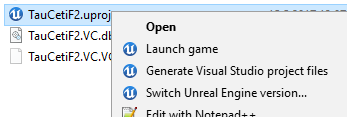
\includegraphics[ width=80mm]{../img/program/generateProjectFiles}

\caption{Vytvoření projektu hry}
\label{fig:generateProjectFiles}

\end{figure}
\FloatBarrier

Tento postup je v~praxi běžně používaný.  Celý projekt je totiž vytvořen na základě informací ze složky \textit{Source}. Mimo jiné má tento přístup tu výhodu, že při použití systému správy verzí (jako například GITu) se tyto vygenerované soubory nemusí verzovat -- každý vývojář si je vytvoří na svém počítači.

Pokud v~kontextové nabídce chybí možnosti pro \UE{}, je potřeba provést asociaci s~\TT{uproject} soubory. Tato asociace by měla být provedena automaticky, nejpozději po vytvoření libovolného \CPP{} projektu z~kterékoliv šablony. Ze zkušenosti autora -- toto se mnohdy nemusí podařit. Pokud se nepodaří vygenerovat projekt hry, může pomoci druhý přístup otevření projektu, který je popsán v~následující části.

Předposledním krokem je v~případě úspěšného vytvoření projektu hry jeho otevření ve \textit{Visual Studiu}, nastavení \textit{TauCetiF2} jako hlavní spustitelnou část projektu (viz obrázek \ref{fig:vs}) a~následné spuštění  editoru hry.


\begin{figure}[!ht]\centering
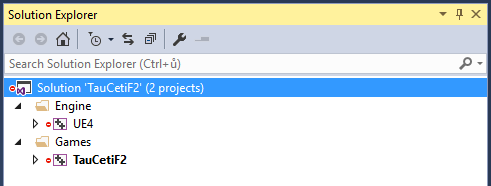
\includegraphics[ width=110mm]{../img/program/vs}

\caption{Vygenerování projektu hry}
\label{fig:vs}

\end{figure}

\FloatBarrier



\subsubsection{Přímé spuštění Editoru}
Druhý postup zahrnuje prosté spuštění Editoru dvojklikem na soubor projektu. Pokud soubor projektu nemá modrou ikonu jako na obrázku \ref{fig:generateProjectFiles}, není tento typ souborů asociovaný s~Unreal Editorem. Pak je nutné otevřít Editor přes \textit{Epic Games Launcher}, najít a~otevřít soubor projektu. Protože hra využívá systému modulů, při prvním spuštění se uživateli zobrazí hláška o~tom, že některé moduly je potřeba zkompilovat. Tuto akci necháme provést. Pokud by kompilace modulů selhala, nejspíše máme problém s~Visual Studiem. V~takovém případě doporučujeme postup níže v~rámci \textit{kroků poslední záchrany}.

Pokud je úspěšně otevřen a~načten Editor, zbývá poslední krok -- výběr obnovy projektu, jak je naznačeno na obrázku \ref{fig:ue_refresh}.

\begin{figure}[!ht]\centering
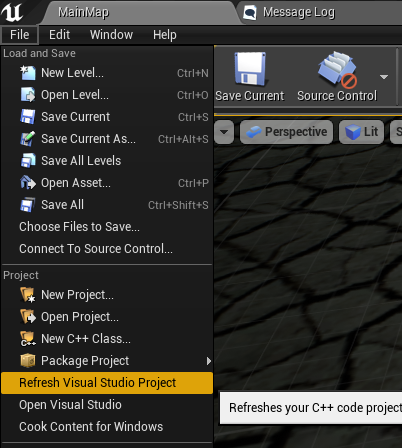
\includegraphics[ width=80mm]{../img/program/ue_refresh}

\caption{Vygenerovaný projekt hry}
\label{fig:ue_refresh}

\end{figure}

\FloatBarrier


\subsubsection{Kroky poslední záchrany}
Pokud všechny námi uvedené postupy selžou, je potřeba si ověřit, že je možné založit libovolný projekt (založený na \CPP{}) z~dodávaných šablon, zkompilovat jej a~vygenerovat projekt pro Visual Studio. Pokud se to povede s~projektem z~nějaké připravené šablony, mělo by to fungovat i~s~naší hrou. V~případě, že ani tento postup nefunguje, je potřeba zjistit příčinu z~kompilačních Logů. Řešení této nefunkčnosti jde mimo téma této práce, takže se jím nebudeme dále zabývat.





